\chapter{Documento de Diseño del Juego (GDD)}
\label{GDD}

\section{Descripción general}
El juego que se pretende desarrollar se basa en el apartado de navegación por el mapa y combate
típicos en los \ac{RTS}. A lo largo de los distintos niveles, el jugador deberá hacer
frente a distintos desafios como pueden ser: escoltar con sus unidades de un punto
del mapa a otro a un personaje importante y/o eliminar a todas las entidades enemigas del escenario.

La ficha técnica es la siguientes:

\begin{itemize}
	\item \textbf{Título:} \placeholdertext{N/A.}
	\item \textbf{Plataforma:} \ac{PC} (Windows y Linux).
	\item \textbf{Género:} \acf{RTS}.
	\item \textbf{Idioma:} Inglés.
	\item \textbf{Clasificación:} PEGI 7\footnote{Web de la asociación https://pegi.info}
\end{itemize}

\section{Mecánicas}
Durante el juego podremos ejecutar una serie de ordenes sobre nuestras unidades para cambiar
su distribución, ordenarles que se desplazen y/o que ataquen a enemigos.\\
Para el desplazamiento por el mapa, el jugador contará con un marcador en el mapa el cual
será capaz de desplazar para que sus unidades lo sigan mientras les sea posible~\ref{fig:mockup_following}.

%El jugador será capaz de seleccionar con el ratón las unidades sobre las que
%quiere lanzar la acción y seleccionar o deseleccionar todas la unidades a su
%disposición mediante atajos de teclado en cualquier momento~\ref{fig:unit-selec} .


%\begin{figure}[ht]
%\centering
%\begin{minipage}[c]{0.45\linewidth}
%	\hspace{1cm}
%	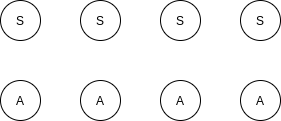
\includegraphics[width=0.7\textwidth]{imagenes/gdd/non-selection.png}
%\end{minipage}
%\begin{minipage}[c]{0.45\linewidth}
%	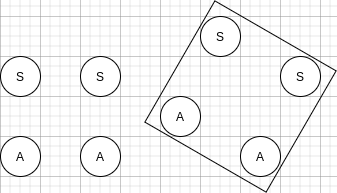
\includegraphics[width=0.7\textwidth]{imagenes/gdd/selection.png}
%\end{minipage}	
%\caption{MockUp selección.}
%\label{fig:unit-selec}
%\end{figure}

\begin{figure}[ht]
\centering
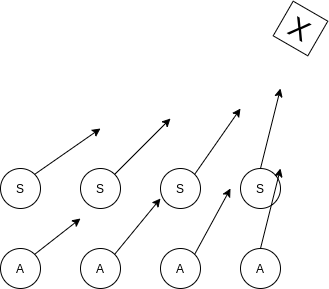
\includegraphics[width=0.35\textwidth]{imagenes/gdd/Following.png}
\caption{MockUp Seguimiento de la marca del jugador.}
\label{fig:mockup_following}
\end{figure}

En cuanto a las posibles formaciones para nuestras unidades, encontramos las siguientes:

\begin{itemize}
\item \textbf{Por filas:}~\ref{mockup_en_fila} las unidades se dispondrán en función de su rango,
siendo encabezado el pelotón por las unidades de ataque a \textit{melee}.

\item \textbf{Sin formación:}~\ref{mockup_desordenada} las unidades no tendrán nigún paramétro de ordenación.

\item \textbf{En anillo:}~\ref{mockup_anillo} formación circular alrededor de una unidad especial. En caso de
no haber unidad escoltada el centro estará vacío. 
\end{itemize} 

\begin{figure}[ht]
\centering
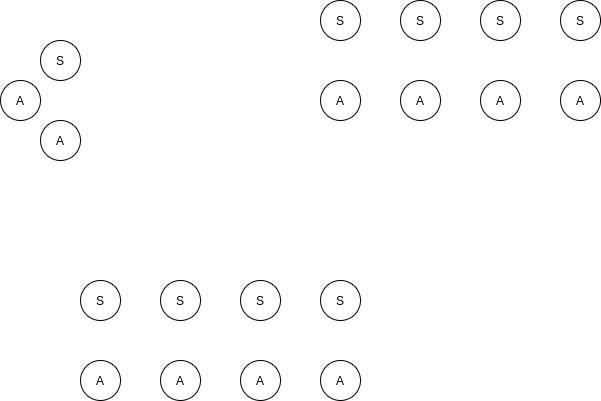
\includegraphics[width=0.45\textwidth]{imagenes/gdd/Formacion-en-fila.png}
\caption{MockUp formacion en fila.}
\label{mockup_en_fila}
\end{figure}

\begin{figure}[ht]
\centering
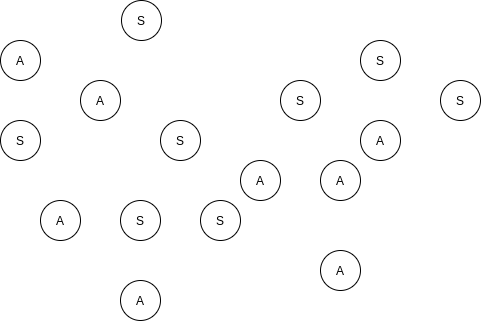
\includegraphics[width=0.45\textwidth]{imagenes/gdd/Formacion-desordenada.png}
\caption{MockUp formacion desordenada.}
\label{mockup_desordenada}
\end{figure}

\begin{figure}[ht]
\centering
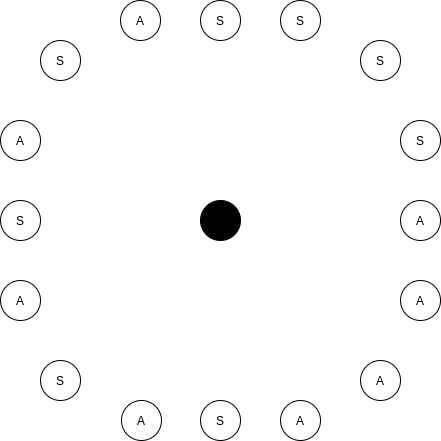
\includegraphics[width=0.3\textwidth]{imagenes/gdd/Formacion-anillo.png}
\caption{MockUp formacion en anillo.}
\label{mockup_anillo}
\end{figure}

%Las acciones posibles serán realizadas en función del objeto y/o lugar donde el jugador haga
%click, si el jugador selecciona una unidad enemiga las unidades marcadas iniciarán un ataque hacía
%esa unidad. Si el objetivo es un punto vacío del mapa, las unidades se desplazarán a el.

Por último podemos ordenar a las unidades que mantengan una estrategia definida:

\begin{itemize}
\item \textbf{Mantener la zona:} en este modo las unidades intentarán evitar dejar su posición
actual, pudiendo desplazarse ligeramente para atacar unidades enemigas. En caso de salir de combate
regresará a su posición.

\item \textbf{Agresivo:} en el momento en el que la tropa divisa un enemigo saldrá diracto a atacarle,
aunque se aleje esta le seguirá mientras siga en su rango de detección.
\end{itemize} 

Aunque el jugador marque una estrategia y forma de plantear el combate, las unidades podrán
decidir si seguir al jugador o revelarse. Si los soldados cercanos están siendo masacrados
existe la posibilidad de que tengan miedo y huyan, si las unidades enemigas nos superan en número
la unidad puede decidir si permanecer en defensa en lugar de atacar de forma activa.

\section{Unidades}
Entre las unidades podemos encontrar dos arquetipos con carácteristicas propias
que nos permitiran crear variedad en las soluciones a la hora de superar el
nivel.

Los tipos son los siguientes:
\begin{itemize}
	\item \textbf{Soldado:} es la unidad más básica que podemos encontrar en el campo de
							guerra, esta armado con una espada y posee estadisticas
							bajas.
	\item \textbf{Arquero:} va equipado con arco y flechas para atacar a distancia a
							sus rivales, tiene menos resistencia que los soldados por
							lo que tendremos que protegerlos para asegurar su
							supervivencia.
\end{itemize}

\begin{center}
\begin{tabular}{|c|c|c|c|}
\hline
        & Daño & Vida & Rango \\ 
\hline
\hline
Soldado & 1    & 5    & Melee \\ 
\hline
Arquero & 2    & 3    & Largo \\ 
\hline
\end{tabular}\\
\placeholdertext{Valores totalmente provisionales}
\end{center}

\section{Controles}
A la hora de jugar tendremos una serie de teclas asignadas a las acciones que el
jugador puede realizar cuando interactúe con el juego. Para enumerarlas dividiremos las
acciones en dos grupos, dependiendo de si son para navegar por los menús o si
representan acciones durante el \textit{gameplay}.

Las teclas para navegar por los menús son las siguientes:

\begin{itemize}
	\item \textbf{Enter:} mediante esta tecla podremos avanzar por los menús una vez estemos sobre la opción deseada.
	\item \textbf{Retroceso:} mediante esta otra podremos ir hacía atrás por los menús.
	\item \textbf{Escape:} esta nos permitirá salir de la ejecución del programa.
	\placeholdertext{igual esto es un poco ilegal.}
\end{itemize}

Las asignadas para jugar son las siguientes:

\begin{itemize}
	\item \textbf{W/A/S/D:} mediante estas teclas podremos desplazar el puntero por el mapa.
	\item \textbf{Barra Espaciadora:} con esta otra podremos ordenar atacar a nuestras unidades,
									  si no encuentran una unidades enemiga en su rango se mantendrá
									  en seguimiento del puntero, si un aliado cercano entra en combate
									  se unirá a la afrenta junto a él.
	\item \textbf{B:} activa el modo huída y las unidades dejarán de combatir y seguirán el
					  puntero aunque tengan enemigos en su campo de visión.									  
\end{itemize}

\section{Pantallas}
Al ejecutar el programa la primera pantalla que aparecerá será la de 
inicio~\ref{mockup_ini}. Se compone del título del juego, la fecha de lanzamiento,
el nombre del desarrollador y un mensaje que nos indica que tenemos que pulsar al tecla
\textit{entre} para continuar, esta pantalla se mantendrá hasta que el jugador presione
dicha tecla.

\begin{figure}[ht]
\centering
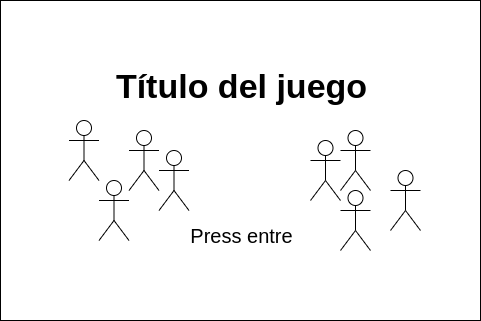
\includegraphics[width=0.45\textwidth]{imagenes/gdd/pantallas/Pantalla_ini.png}
\caption{MockUp pantalla de inicio.}
\label{mockup_ini}
\end{figure}

Una vez pulsado el botón indicado se procederá a cargar el juego mientras se muestra
una barra que indica el progreso de cargado~\ref{mockup_carga}.

\begin{figure}[ht]
\centering
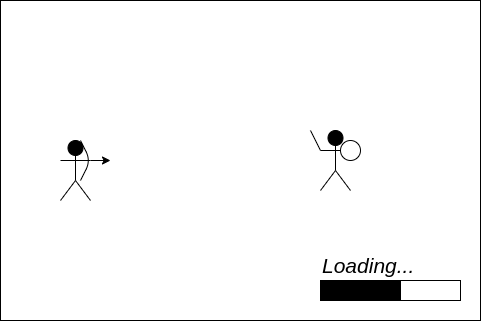
\includegraphics[width=0.45\textwidth]{imagenes/gdd/pantallas/Pantalla_carga.png}
\caption{MockUp pantalla de carga.}
\label{mockup_carga}
\end{figure}

A continuación de la carga pasaremos directamente al escenario, donde se desarrollará el
\textit{gameplay} y nos mantendremos en esta pantalla hasta que termine el juego, ya sea
por victoria o derrota del jugador~\ref{mockup_juego}.

\begin{figure}[ht]
\centering
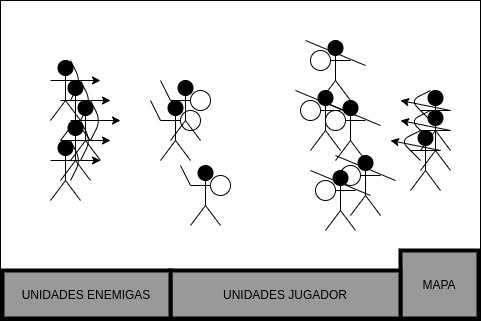
\includegraphics[width=0.45\textwidth]{imagenes/gdd/pantallas/Pantalla_gameplay.png}
\caption{MockUp escenario juego.}
\label{mockup_juego}
\end{figure}

El final de la partida nos trae dos posibles escenarios, la victoria y la derrota. 
Para cada uno saldrá su respectivo mensaje~\ref{mockup_victoria}~\ref{mockup_derrota}
y pasado un momento se nos mandará automáticamente a la pantalla de
inicio~\ref{mockup_ini}.

\begin{figure}[hb]
\centering
\begin{minipage}[c]{0.45\linewidth}
	\hspace{9mm}
	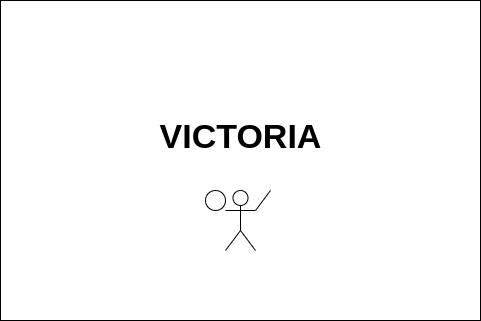
\includegraphics[width=0.7\textwidth]{imagenes/gdd/pantallas/Pantalla_victoria.png}
	\caption{MockUp victoria.}
	\label{mockup_victoria}
\end{minipage}
\begin{minipage}[c]{0.45\linewidth}
	\hspace{9mm}
	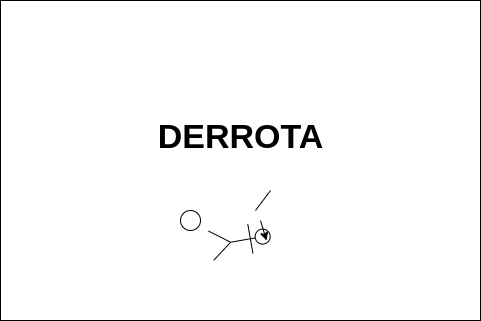
\includegraphics[width=0.7\textwidth]{imagenes/gdd/pantallas/Pantalla_derrota.png}
	\caption{MockUp derrota.}
	\label{mockup_derrota}
\end{minipage}	
\end{figure}

Como última pantalla con la que el jugador podrá interactuar es la del menú de
pausa~\ref{mockup_pausa}, en el cual se le dará la opción de salir o de volver a la
partida, mientras esta pantalla este activa la acción en el juego se paralizará hasta
que el jugador decida. 

\begin{figure}[ht]
\centering
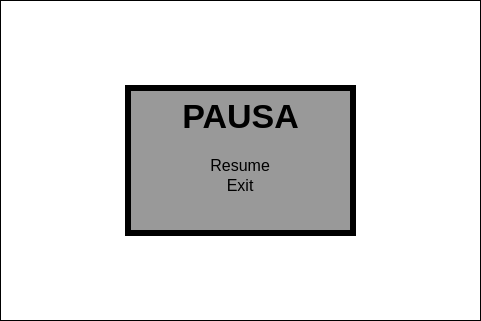
\includegraphics[width=0.45\textwidth]{imagenes/gdd/pantallas/Pantalla_pausa.png}
\caption{MockUp menú de pausa.}
\label{mockup_pausa}
\end{figure}

\section{Estados del juego}
Una vez mostradas todas las posibles pantallas con las que podrá interactuar el jugador,
es interesante dibujar un diagrama de flujo que plasme sus conexiones y posibilidades
con el fin de crear una representación gráfica que sirva como esquema global.

Dicho esquema podemos encontrarlo en la figura~\ref{esq:flow_juego}.

\begin{figure}[ht]
\centering
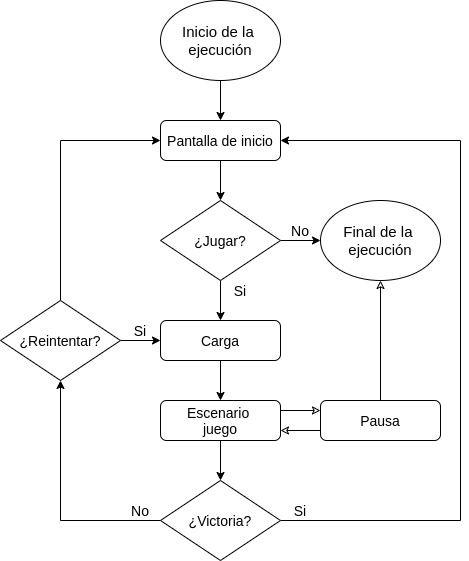
\includegraphics[width=0.45\textwidth]{imagenes/gdd/pantallas/flow_ejecucion.png}
\caption{MockUp flujo de ejecución.}
\label{esq:flow_juego}
\end{figure}

\section{Escenarios}
A lo largo de los niveles la intención es que nos encontremos con distintos biomas como
pueden ser praderas, bosque o desiertos como los que podemos encontrar en \ac{AoE} II
~\ref{img:aoe_2}~\ref{img:mapa_aoe1}~\ref{img:mapa_aoe2}.

\begin{figure}[ht]
\centering
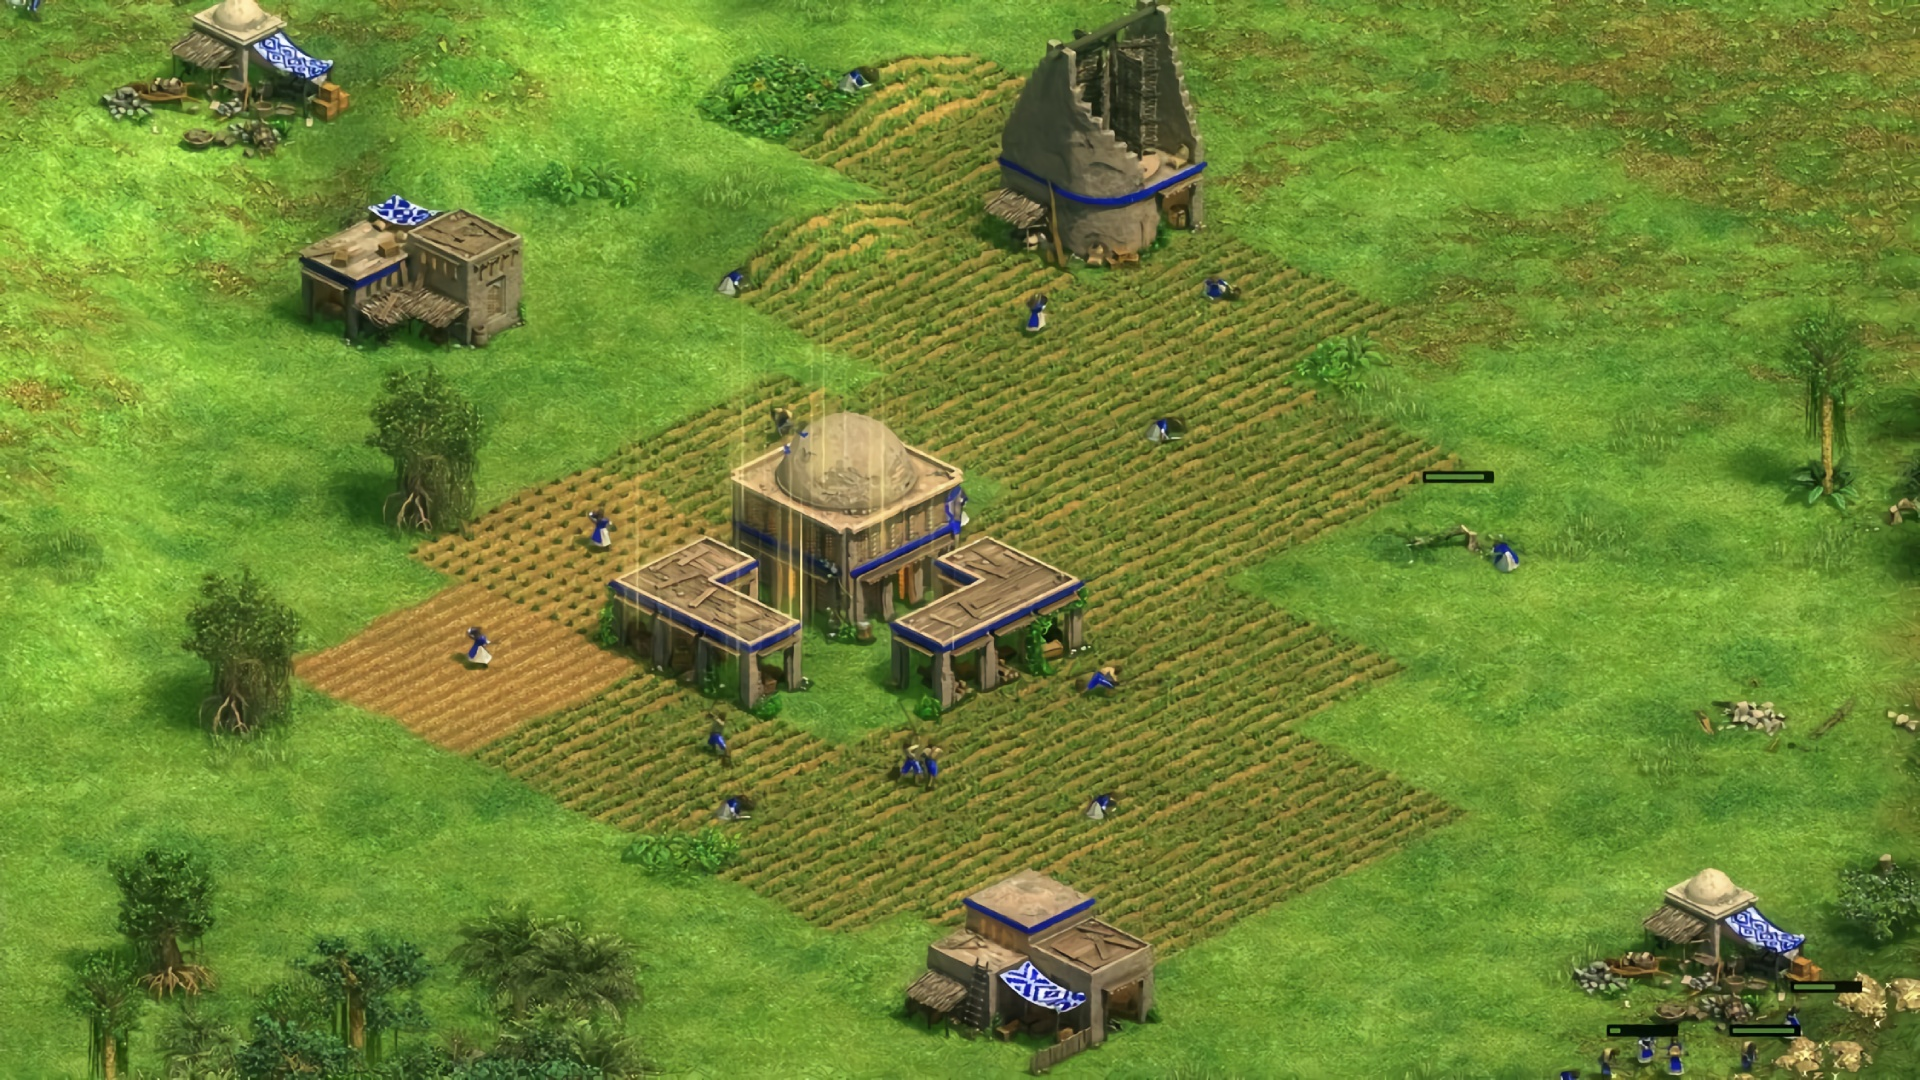
\includegraphics[width=0.6\textwidth]{imagenes/gdd/mapa_aoe_1.jpg}
\caption{Ejemplo escenario con vegetación.}
\label{img:mapa_aoe1}
\end{figure}

\begin{figure}[ht]
\centering
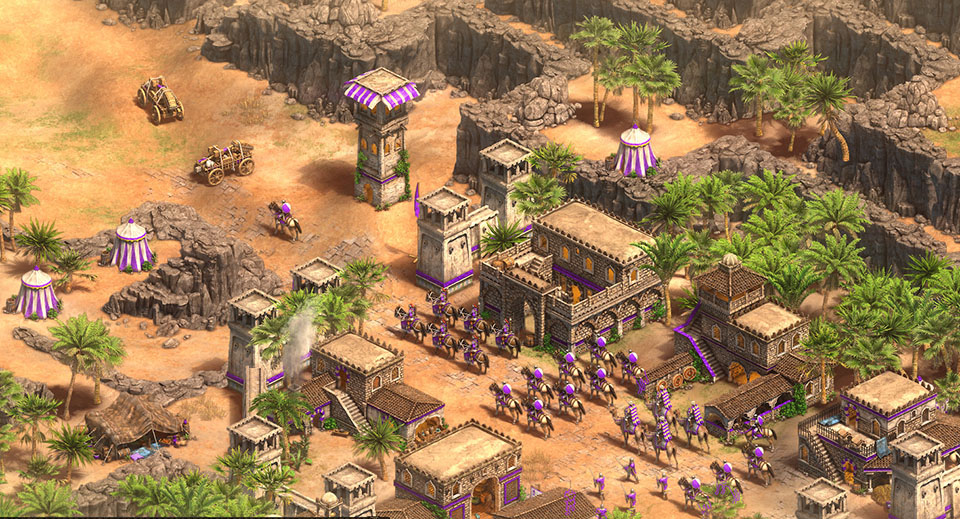
\includegraphics[width=0.6\textwidth]{imagenes/gdd/mapa_aoe_2.jpg}
\caption{Ejemplo escenario desértico.}
\label{img:mapa_aoe2}
\end{figure}

Además de imitar el estilo artístico el juego se desarrollará empleando una cámara
aerea fija manteniendo una perspectiva isométrica que nos permitirá visualizar desde
un punto elevado una gran porción del escenario, esto lo haremos con el fin de dar al
jugador la posibilidad de conocer lo máximo posible el territorio cercano posible y a la
vez le libramos de tener que estar preocuparse de situar la cámara para cada momento. \\
Al mantener una posición fija podemos situar todos los elementos en la escena de forma
que no obstaculicen la visión o molesten al jugador.

\section{Mínimo producto viable}
Una vez planteadas todas las características deseadas para el videojuego, es acosenjable
decidir que partes del producto son vitales para mostrar la experiencia
de juego deseable, el hecho de marcar estos objetivos nos ayudará a poder desarrollar una
versión reducida del proyecto que nos permita dar la sensación de tener un producto acabado.\\
Es importante realizar este proceso ya que por motivos internos o externos al equipo de desarrollo,
siempre existen contratiempos que nos impidan conseguir todos los objetivos propuestos en el
documento.

En cuanto a las etapas en la ejecución del juego, encontramos esencial el poder finalizar el nivel,
ya sea por victoria o derrota. Acto seguido volver al comienzo del nivel, dejando a un lado un
posible menú inicial y de pausa.

Una vez en partida el juego constará de un nivel único compuesto por: un escenario estático
mínimo, un conjunto de unidades propiedad del jugador y otro perteneciente a la máquina.\\
Al inicio del juego el jugador se encontrará quieto en uno de los extremos del nivel y el enemigo 
estará patrullando por una zona designada, dejando así a elección del jugador la distribución y el
momento exacto en el que comenzará la disputa.

En lo referente a las mecánicas y jugabilidad, es importante que el jugador sea capaz de poder
mover a sus unidades por el escenario y ordenarles atacar, por otro lado sería deseable poder
ajustar algunos parámetros del comportamiento de su ejercito para poder pasar el nivel de más
de una forma.\\
Otro lado la \ac{IA} debe ser capaz de detectar el acercamiento del jugador y responder a la
ofensiva, dejando la capacidad de tomar la iniciativa y variar su estrategia para versiones
más completas. Ambos ejercitos se compondrán de soldados y arqueros.

En lo referente al apartado visual, sería deseable tener sprites para unidades y escenario pero
de ser necesario podemos mantener el sistema de \textit{render} inicial.
